\documentclass[11pt, a4paper]{article}
\usepackage{threeparttable} % Add this to your preamble

\usepackage{parselines} 
\usepackage{graphicx}
\usepackage{helvet}
\usepackage[utf8]{inputenc}
\renewcommand\familydefault{\sfdefault}
\usepackage{pgfgantt}       % Pour les diagrammes de Gantt
\usepackage{pdflscape}
\usepackage{url}
\usepackage{makecell}
\usepackage{wrapfig}
\usepackage{xcolor}
\usepackage{listings}
\usepackage{amsfonts}
\usepackage{multicol}
\usepackage{mathtools}
\usepackage{amsmath}
\usepackage{float}
\newcommand{\bigzero}{\mbox{\normalfont\Large\bfseries 0}}
\newcommand{\rvline}{\hspace*{-\arraycolsep}\vline\hspace*{-\arraycolsep}}

\usepackage[linesnumbered,ruled,vlined]{algorithm2e}
\usepackage[colorlinks=true,hyperfootnotes=false,citecolor=blue]{hyperref}
\usepackage[capitalise]{cleveref}
\usepackage{siunitx}
\usepackage{todonotes}
\usepackage{cite}
\usepackage{comment}
\usepackage{booktabs}
\usepackage{multirow}
\usepackage{tabularray}
\UseTblrLibrary{booktabs}
\usepackage{caption}
\usepackage{setspace}

\usepackage{geometry}
\usepackage{tabularx}
\usepackage{enumitem}
\usepackage[table, dvipsnames]{xcolor}
\usepackage[utf8]{inputenc}
\usepackage[T1]{fontenc}
\usepackage{lmodern}
\usepackage{amsmath}

\pagestyle{empty}

\geometry{a4paper, margin=1in}

\ganttset{group/.append style={orange},
milestone/.append style={red},
progress label node anchor/.append style={text=red}}

\usepackage{multicol}
\usepackage{titlesec}

\titleformat{\section}{\large\bfseries}{\thesection}{1em}{}
\titlespacing*{\section}{0pt}{1ex}{1ex}

\usepackage{tikz}
\usetikzlibrary{shapes.geometric, arrows}
\tikzstyle{startstop} = [rectangle, rounded corners, minimum width=3cm, minimum height=1cm,text centered, draw=black, fill=red!30]
\tikzstyle{process} = [rectangle, minimum width=3cm, minimum height=1cm, text centered, draw=black, fill=blue!20]
\tikzstyle{arrow} = [thick,->,>=stealth]

\usepackage{enumitem}
\setlist[enumerate]{itemsep=0pt, parsep=0pt, topsep=0pt}
\setlist[itemize]{itemsep=0pt, parsep=0pt, topsep=0pt}



\begin{document}

\title{Launching Packages 2025~\\Protecting Software and  Hardware Implementations}
\author{Gustavo Banegas~\\
 INRIA \& LIX, École Polytechnique~\\
 gustavo.souza-banegas@polytechnique.edu}
\date{}
\maketitle

\section{Résumé du Scientifique}
%\begin{enumerate}
%    \item \textbf{Le résumé du scientifique} (3 pages max.) mettant en avant les rubriques suivantes, en lien avec les critères d’évaluation :
%    \begin{itemize}
%        \item \textbf{Présentation} : positionnement, enjeux, objectifs, méthodes, liens avec la stratégie de l’École.
%        \item \textbf{Impacts, retombées et ambitions} : publications, colloques, collaborations, contrat industriel, obtention de financement (ERC, ANR, …).
%    \end{itemize}
%\end{enumerate}

With the advent of quantum computers capable of running Shor's 
algorithm~\cite{365700}, currently deployed public-key 
cryptography \textbf{will be catastrophically and irreversibly broken}, 
exposing all past and future encrypted communications. 
This risk has pushed a global initiative to develop cryptographic 
systems resistant to quantum attacks, known as Post-Quantum Cryptography (PQC). 
Research in PQC has intensified, particularly following 
\href{https://csrc.nist.gov/projects/post-quantum-cryptography/post-quantum-cryptography-standardization/call-for-proposals}
{the launch of the United States National Institute of Standards and Technology (NIST) PQC standardization project in 2016}
and the ongoing call in 2023 of \href{https://www.nist.gov/news-events/news/2023/07/nist-announces-additional-digital-signature-candidates-pqc-standardization}
{NIST's additional digital signature candidates}.
However, participation in this project is global, and most countries follow its standards (including 
the European Union).

The development of cryptographic schemes follows a structured process: (1) It begins with the establishment of computational hardness assumptions through 
mathematical analysis, providing the theoretical foundation for security.
(2) These foundations enable the design of cryptographic primitives that leverage secure trapdoor functions, 
forming the basis of new encryption and signature schemes.
(3) Once the theoretical groundwork is laid, algorithms are formally specified and prototyped, leading to 
reference implementations. 
(4) The final stage involves integrating these solutions into real-world applications, ensuring their adoption 
through production-ready implementations.


The first international PQC standards were published last year
with \href{https://csrc.nist.gov/pubs/fips/204/final}{ML-DSA} 
(signature scheme) and \href{https://csrc.nist.gov/pubs/fips/203/final}{ML-KEM} 
(encryption scheme), 
however, post-quantum cryptography remains an 
active research area with \emph{critical challenges}. 
Improving efficiency and \textbf{hardening implementations against side-channel attacks (SCA)} 
have become \textbf{crucial}. As PQC transitions from theory to practice, 
its security in real-world deployments depends not 
only on its mathematical foundations but also on its 
resilience to physical attacks. Strengthening implementations against 
SCA is mandatory to prevent adversaries from extracting secret 
information through power analysis, electromagnetic leakage, or 
fault injection. This aspect of PQC is essential for secure adoption 
in applications such as hardware security modules, IoT devices, and 
vehicular communication---where attackers have physical access and 
SCA defenses are not optional but necessary.

\textbf{The goal of this project is to ensure cryptographic security beyond mathematical 
guarantees by evaluating and strengthening its resistance to physical attacks.}

\subsection*{Security Analysis of Post-Quantum Schemes}\label{sec:an}\vspace{-0.1cm}

Cryptosystems face vulnerabilities to SCA, wherein an adversary can deduce 
confidential information from physical observations--such as timing,
electromagnetic emanation, or power consumption--made during the execution of 
computations using sensitive data~\cite{brumley2005remote, KocherJJR11,10.1007/3-540-48405-1_25}.
These attacks can be classified as passive, where the a
dversary simply observes leaked information without interfering, or active, 
where faults are intentionally injected to manipulate computations and extract 
secrets~\cite{4599557,6076462}. Both types pose serious threats and have been successfully employed 
across various applications, often proving challenging to detect.

Exploring SCA requires specialized equipment and training, as the 
methodologies and countermeasures are highly dependent on the 
targeted cryptosystem. While techniques exist to mitigate these 
attacks, many are intrinsic to specific schemes and lack easy 
adaptability to others. Consequently, securing each implementation 
demands a unique approach, necessitating expertise in both 
cryptographic engineering and side-channel analysis. Unfortunately, 
the pool of individuals capable of combining these essential skills 
remains limited to a select group of professionals. Based on my experience in the 
security architecture industry, there is a 
clear shortage of professionals with the necessary expertise in this 
field. We aim to give a first step to develop the knowledge
and foundation for training students in hardware security.
\vspace{-0.5cm}


\paragraph{Methodology.} This project comprises three 
interdependent phases designed to bridge gaps 
in hardware security and achieve practical implementation robustness:


\begin{enumerate}
\item \textbf{Enumerate Attack Surfaces and Analyze Vulnerabilities} 
\begin{itemize}[leftmargin=2em] 
\item Investigate cryptographic targets: 
\begin{itemize} \item USA NIST PQC candidates 
(\href{https://csrc.nist.gov/projects/post-quantum-cryptography/round-4-submissions}{Round 4}, 
\href{https://csrc.nist.gov/projects/pqc-dig-sig/round-2-additional-signatures}{Additional Call}) 
\item \href{https://www.kpqc.or.kr/competition.html}{Korean PQC} 
\item \href{https://niccs.org.cn/en/notice/}{China PQC} 
\end{itemize} 
\item Assess vulnerabilities using Husky and CW-Lite boards; 
\item Execute attack: 
    \begin{itemize} 
    \item \textit{Passive}: Perform time analysis and Differential Power Analysis (DPA) 
    \item \textit{Active}: Apply clock/voltage glitching 
    \end{itemize} 
\end{itemize}

\item \textbf{Prototype Adaptive Countermeasures}
\begin{itemize}[leftmargin=2em]
    \item Develop algorithm-aware protection strategies:
    \begin{itemize}
        \item Implement masking techniques to obscure sensitive data without efficiency loss
        \item Design fault-tolerant operations to resist induced faults
    \end{itemize}
    \item Deploy countermeasures across platforms:
    \begin{itemize}
        \item Integrate software protections on embedded systems (Cortex-M4/M3)
        \item Implement hardware mitigations in FPGA architectures
    \end{itemize}
\end{itemize}

\item \textbf{Validate Implementations and Benchmark Security}
\begin{itemize}[leftmargin=2em]
    \item Test software countermeasures on Cortex-M3/M4 processors
    \item Verify hardware countermeasures using PolarFire and Xilinx FPGAs
    \item Quantify security improvements:
    \begin{itemize}
        \item Measure side-channel resistance: Practical approach and Test Vector Leakage Assessment (TVLA)
        \item Assess computational overhead: Cycle count analysis vs. baseline specifications
    \end{itemize}
\end{itemize}
\end{enumerate}
The research \textbf{fills a significant gap}, as LIX does not yet have 
the materials nor the expertise in hardware security. 
Validation is crucial to ensure that the developed countermeasures 
are both practical and effective. The project will be strengthened by 
leveraging my industrial experience and collaborations. 
A PhD student will be hired to work on side-channel analysis and 
cryptographic hardware security, contributing across all three 
research areas: (1) identifying vulnerabilities, (2) designing and 
implementing countermeasures, and (3) validating security 
enhancements.

\vspace{-0.5cm}

%\subsection*{Impacts and Outcomes}

\paragraph{Impacts on Institute Polytechnique de Paris (IPP).}
This project introduces a new research topic in hardware security, 
aligning with the objectives of the cybersecurity program at 
EPP. 
The program aims to equip students with expertise in 
cryptographic security, hardware security, and side-channel analysis. 
By fostering research and innovation in these critical areas, 
it contributes to the development of next-generation security 
professionals capable of addressing emerging threats in 
cryptography and beyond. Given the strong demand for expertise 
in this field, this initiative will play a crucial role in knowledge 
dissemination, training, and academic collaborations. Moreover, the 
project will be carried out within the new research team \'Eclair, 
where early support will help build a base for further developments, 
including lab projects and contributions to the Cybersecurity 
Master's program.

\paragraph{Publications and scientific outcome.} Targeting top-tier cryptography and security conferences and journals such as 
\href{https://ches.iacr.org/index.php}{CHES}, \href{https://eurocrypt.iacr.org/}{EUROCRYPT}, 
\href{https://asiacrypt.iacr.org/}{ASIACRYPT}, 
\href{https://ieeexplore.ieee.org/xpl/RecentIssue.jsp?punumber=10206}{IEEE Transactions on Information Forensics and Security}, 
and the \href{https://link.springer.com/journal/13389}{Journal of Cryptographic Engineering}. 

\vspace{-0.5cm}
\paragraph{Scientific Collaborations.} Engaging in academic collaborations with international 
researchers, including \href{https://mtrimoska.com/}{Monika Trimoska} (TU/e, Netherlands),
\href{https://www.sopmac.de/index.html}{Fábio Campos}(H-BRS, Germany), \href{https://research.aalto.fi/en/persons/chris-brzuska}{Chris Brzuska} (Aalto, Finland) 
and Łukasz Chmielewski (Masaryk University, Czech Republic). 
%with other international researchers like \href{https://research.aalto.fi/en/persons/chris-brzuska}{Chris Brzuska} (Aalto, Finland) 
%early-career researchers, including \href{https://mtrimoska.com/}{Monika Trimoska} (TU/e, Netherlands) and 
%\href{https://www.sopmac.de/index.html}{Fábio Campos}(H-BRS, Germany), as well as continuing partnerships 
%with other international researchers like \href{https://research.aalto.fi/en/persons/chris-brzuska}{Chris Brzuska} (Aalto, Finland) 
%and Łukasz Chmielewski (Masaryk University, Czech Republic). Additionally, initiating a project with local researcher Guénaël Renault. 
%Participation in research workshops and summer schools, such as the 
%\href{https://summerschool-croatia.cs.ru.nl/}{Summer School on Real-World Cryptography and Privacy}, 
%is also planned.
\vspace{-0.5cm}


\paragraph{Industrial Impact.}
Drawing on my experience at 
\href{https://www.qualcomm.com/}{Qualcomm}, this project tackles 
the shortage of experts in assessing physical threats to 
cryptography. The industry needs specialists who bridge 
theoretical security with practical implementation, especially in 
embedded systems and hardware-based cryptography. By collaborating 
with industry leaders like NXP and Thales, we aim to develop 
expertise for real-world security challenges and translate 
cutting-edge research into practical countermeasures. Additionally, 
through the \href{https://quantique.france2030.gouv.fr/recherche-innovation/projets-de-cryptographie-post-quantique/}
{Bpifrance HYPERFORM consortium}, my group gains
direct access to industrial challenges in the first year.
\vspace{-0.5cm}



%Establishing connections with industry, 
%particularly in embedded security and hardware-based cryptographic 
%implementations, to evaluate the practical adoption of countermeasures. 
%My experience at \href{https://www.qualcomm.com/}{Qualcomm} provides a 
%strong foundation for building future collaborations. Additionally, I 
%have connections with professionals such as Matthieu Rivain and Sonia 
%Belaïd from \href{https://www.cryptoexperts.com/people/}{CryptoExperts}, 
%as well as Christine Cloostermans at 
%\href{https://www.nxp.com/company/about-nxp/smarter-world-blog/BL-EMBRACING-EQUITY-ON-EVERY-LEVEL}{NXP}, 
%facilitating real-world feedback and further industrial partnerships.


%Moreover, other satellite 
%conferences, such as \href{https://cascade-conference.org/cfp.html}{CASCADE}, also 
%focus on related topics.

%\paragraph{Scientific Collaborations.} Engaging in academic collaborations with international 
%early-career researchers, including \href{https://mtrimoska.com/}{Monika Trimoska} (TU/e, Netherlands) and 
%\href{https://www.sopmac.de/index.html}{Fábio Campos}(H-BRS, Germany), as well as continuing partnerships 
%with other international researchers like \href{https://research.aalto.fi/en/persons/chris-brzuska}{Chris Brzuska} (Aalto, Finland) 
%and Łukasz Chmielewski (Masaryk University, Czech Republic). Additionally, initiating a project with local researcher Guénaël Renault. 
%Participation in research workshops and summer schools, such as the 
%\href{https://summerschool-croatia.cs.ru.nl/}{Summer School on Real-World Cryptography and Privacy}, 
%is also planned.

\paragraph{Funding Prospects.}The plan is to set up this project and acquire 
the necessary materials to consolidate the results and prepare an application for 
European Research Council (ERC) funding in 2026. The deadline for the Starting Grant is July 2026.
The development and submission of this proposal is included in the project calendar below.
%The plan is to establish this project, 
%set up the necessary equipment, consolidate the results, 
%and then prepare an application for funding from the E
%uropean Research Council (ERC) and the French National 
%Research Agency (ANR). This proposal will also support the formation of 
%a new group, Éclair, which originates from the former GRACE team.




%\begin{figure}
%\begin{center}
%\resizebox{.5\textwidth}{!}{
%\framebox{
%    \begin{tikzpicture}[node distance=2cm]

        % Nodes
%        \node (start) [startstop] {Research Start};
%        \node (evaluate) [process, below of=start] {Evaluate Side-Channel Attacks (Identify Vulnerabilities)};
%        \node (design) [process, below of=evaluate] {Design Countermeasures (Masking, Blinding, Fault Detection)};
%        \node (benchmark) [process, below of=design] {Benchmark \& Validation (Security, Performance Trade-offs)};
%        \node (end) [startstop, below of=benchmark] {Conclusions \& Future Work};

        % Arrows
%        \draw [arrow] (start) -- (evaluate);
%        \draw [arrow] (evaluate) -- (design);
%        \draw [arrow] (design) -- (benchmark);
%        \draw [arrow] (benchmark) -- (end);

%    \end{tikzpicture}
%    }
%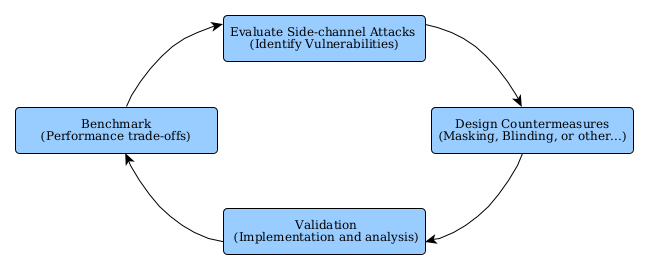
\includegraphics[scale=0.4]{cycle.png}
%%\caption{Overview of the methdology for the project.}
%\label{fig:methodology}
%\end{center}
%\end{figure}



%Fortunately, I have honed these skills throughout my career as a researcher and developed hardware 
%proficiency during my tenure at Qualcomm, a leading semiconductor design company. Additionally, I 
%possess knowledge of emerging threats to cryptography, including security analyses leveraging 
%quantum algorithms. Even with NIST moving to 
%\href{https://csrc.nist.gov/Projects/post-quantum-cryptography/round-4-submissions}{Round 4},
%\footnote{\url{https://groups.google.com/a/list.nist.gov/g/pqc-forum/c/fvnhyQ25jUg/m/NJzYDqQBBAAJ}} current 
%submissions are still open to scrutiny, and may be subject to theoretical attacks (where one can break the entire 
%scheme) and side-channel attacks. The whole scientific community can propose attacks and/or improvements for 
%the submissions, to make the schemes more robust. I am therefore particularly interested in doing this.  
%Specifically, I am currently working on \textbf{evaluating security against side-channel attacks} and 
%\textbf{studying quantum algorithms}, to harden PQC algorithms.



\subsubsection*{Budget}

%Table \ref{tab:hardware_components} details the essential 
%%equipment required for comprehensive security evaluation of 
%post-quantum cryptographic implementations. The hardware 
%selection addresses three critical operational needs: 
%(1) precise side-channel measurement capabilities, (2)
% target device programmability for various cryptographic schemes, 
% and (3) high-speed signal acquisition infrastructure.

\begin{table}[H]
\centering
\caption{Budget for hardware equipment.}
\label{tab:hardware_components}
\resizebox{0.8\textwidth}{!}{%
\begin{tabular}{|l|p{8cm}|c|c|l|}
\toprule
\textbf{Hardware} & \textbf{Usage} & \textbf{Qty} & \textbf{Total Price} (€) & \textbf{Link} \\ \midrule
Husk Board & Side-channel acquisition / fault attack & 2 & €$1\,060$ & \href{https://www.mouser.fr/ProductDetail/NewAE/NAE-CWHUSKY-SK1?qs=rQFj71Wb1eUq6zUbSt2x8g\%3D\%3D}{Mouser} \\ \hline
Server & Run analysis and store the data acquired by the boards. & 1 & €$3\,300$ & \\ \midrule
Polarfire FPGA & Development of specific hardware for cryptography & 1 & €$150$ & \href{https://www.microchip.com/en-us/development-tool/mpfs-disco-kit}{Microchip} \\ \midrule
Arty S7: Spartan-7 FPGA & Development of specific hardware for cryptography & 1 & €$300$ & \href{https://digilent.com/shop/arty-s7-spartan-7-fpga-development-board/}{Digilent} \\ \midrule
CW-lite ARM & Small ARM board for side-channel attacks & 2 & €$700$ & \href{https://www.newae.com/products/nae-cwlite-arm}{NewAE} \\ \midrule
Nucleo ARM & Board with Cortex-M3/M4 (NUCLEO-F207ZG/NUCLEO-L4R5ZI) & 4 & €$400$ & \href{https://www.mouser.fr/}{Mouser}\\ \midrule
PicoScope 3000E & Oscilloscope (Data acquisition) & 1 & €$4\,655$ & \href{https://www.picotech.com/oscilloscope/picoscope-3000e-series-500-mhz-5gs-digital-usb-oscilloscope?model=3418E}{PicoTech} \\ \midrule
Wires / Cables / Others & Connection with oscilloscope, soldering kit, etc. & 1 & €$700$ & \\ \bottomrule
$--$ & $--$ & $--$ & €$11\,235$  & $--$ \\
\bottomrule
\end{tabular}%
}
\end{table}

%The \emph{PhD student position} is planned for a duration of three years, with a total 
%salary of €75,000. Additionally, we have allocated 
%€4,000 per year for the student to attend international 
%conferences such as Eurocrypt and CHES, as well as summer schools. 
%This brings the total estimated cost to €87,000.

%Regarding internship opportunities, we can host master's 
%students for six-month projects. The main goal is to familiarize them 
%with side-channel attacks through smaller projects, such as data 
%acquisition and analysis or the implementation of countermeasures for 
%cryptographic schemes. For such, X will be destinated 
%to pay for the internship.


%Therefore, the total estimated cost for the PhD student is €87,000,
%the costs for internship is estimated in X, 
%and the overall project cost, including equipment, is €97,635 + X. FIXME


\begin{table}[H]
    \centering
    \caption{Budget Breakdown}
    \resizebox{0.6\textwidth}{!}{%
    \begin{threeparttable}
    \begin{tabular}{|ll|l|}
        \toprule
        \textbf{Category} & \textbf{Details} & \textbf{Amount} (€) \\
        \midrule
        \multirow{3}{*}{Personnel} 
            & 1 PhD & €$157$K\tnote{a}\\
            & 2 x 6-month M2 interns (40h/week) & €$8\,352$\tnote{b}\\
        \midrule
        \multirow{2}{*}{Equipment} 
            & Hardware & €$11\,235$ \\
            & Laptop for PhD & €$3$K \\
        \midrule
        \multirow{3}{*}{Travel} 
            & International conference (Overseas) & €$3$K/year \\
            & International conference (Europe) & €$2$K/year \\
            & National workshops \& seminars & €$1$K/year \\
        \midrule
        \textbf{Total} &  & €$197\,587$ \\
        \bottomrule
    \end{tabular}
    \begin{tablenotes}
    \item[a]PhD student starting in 2025 is €$157\,000$, and it will rise to €$163\,500$ for a thesis starting in 2026.
    \item[b] According to the IPP: For trainees, the minimum remuneration is $4.35$ euros per hour, with no additional charge.
    \end{tablenotes}
    \end{threeparttable}
    }
    \label{tab:budget}
\end{table}
%\newpage
\begin{landscape}

\section{Calendar}
\begin{ganttchart}[%Specs
     y unit title=0.5cm,
     y unit chart=0.7cm,
     vgrid,hgrid,
     title height=1,
%     title/.style={fill=none},
     title label font=\bfseries\footnotesize,
     bar/.style={fill=blue},
     bar height=0.7,
%   progress label text={},
     group right shift=0,
     group top shift=0.7,
     group height=.3,
     group peaks width={0.2},
     inline]{1}{36}
    %labels
    %\gantttitle{A three-years project}{36}\\  % title 1
    \gantttitle[]{2025}{6}                 % title 2
    \gantttitle[]{2026}{12} 
    \gantttitle[]{2027}{12}
    \gantttitle[]{2028}{6}\\              
 %   \gantttitle{Q1}{3}                      % title 3
 %   \gantttitle{Q2}{3}
    \gantttitle{Q3}{3}
    \gantttitle{Q4}{3}
    \gantttitle{Q1}{3}
    \gantttitle{Q2}{3}
    \gantttitle{Q3}{3} 
    \gantttitle{Q4}{3}
    \gantttitle{Q1}{3}
    \gantttitle{Q2}{3}
    \gantttitle{Q3}{3} 
    \gantttitle{Q4}{3}
    \gantttitle{Q1}{3}                      % title 3
    \gantttitle{Q2}{3}    \\
    % Setting group if any
   % \ganttgroup[inline=false]{Group 1}{1}{5}\\ 
    \ganttbar[inline=false]{Selection of candidates}{1}{4}\\
    \ganttbar[inline=false]{Acquiring equipment}{3}{5}\\
    \ganttbar[inline=false]{Evaluation of candidates}{5}{10}\\
    \ganttbar[inline=false]{Development of attacks}{6}{12}\\
    \ganttbar[inline=false, bar/.append style={fill=teal}]{Intership Master M2}{5}{11}\\
    %\ganttbar[inline=false]{Writing of the attack}{10}{11}\\
    \ganttmilestone[inline=false]{1st Publication (Journal)}{13} \\
    \ganttbar[inline=false, bar/.append style={fill=purple}]{Writing application for ERC}{9}{12} \\
    \ganttmilestone[inline=false, milestone/.append style={fill=green}]{Deadline Submittion ERC 2026}{12} \\
    \ganttbar[inline=false]{Development of the countermeasure}{11}{16}\\
    \ganttbar[inline=false]{Implementation of the countermeasure}{13}{19}\\
    \ganttbar[inline=false, bar/.append style={fill=teal}]{Intership Master M2}{13}{19}\\
    \ganttbar[inline=false]{Evaluation of the countermeasure}{16}{19}\\
    \ganttbar[inline=false]{Scentific write of the framework}{15}{22}\\
    \ganttmilestone[inline=false]{2nd publication (CHES)}{20} \\
    \ganttbar[inline=false]{Evaluation of hardware design }{20}{26}\\
    \ganttbar[inline=false]{Prototype of secure hardware}{22}{32}\\
    \ganttbar[inline=false]{Evaluation of secure techniques}{26}{34}\\
    \ganttmilestone[inline=false]{3nd publication (CHES/Eurocrypt)}{35} \\
    %\ganttbar[inline=false]{Preparatiof for the defense}{33}{36}\\
    %\ganttmilestone[inline=false]{PhD Thesis Defense}{36} \\ 
\end{ganttchart}
\end{landscape}


\newpage
%\section{CV}
%\begin{enumerate}
%    \item The scientific summary (maximum 3 pages) highlighting the following sections, in connection with the evaluation criteria:
%    \begin{itemize}
%        \item \textbf{Presentation:} positioning, challenges, objectives, methods, links with the School's strategy.
%        \item \textbf{Impacts, outcomes, and ambitions:} publications, conferences, collaborations, industrial contracts, funding acquisition (ERC, ANR, ...).
%    \end{itemize}
    
%    \item The timeline detailing the work plan over 3 years (maximum 1 page).
%    
%    \item The projected budget over 3 years (maximum 1 page). This budget must be realistic, and the Foundation reserves the right to suspend or even terminate the project's funding, particularly in the event of an unjustified failure to comply with the budget.
    
%    \item The candidate's CV (maximum 3 pages).
%\end{enumerate}

\subsection*{CV - Gustavo Banegas}
Current position: INRIA Inria Starting Faculty Position \& Chargé d'Enseignement in Computer Science, École Polytechnique ~\\
\href{www.cryptme.in}{Personal Webpage}~\\
gustavo.souza-banegas@polytechnique.edu~\\

\subsection*{Professional Experience}
\resizebox{\linewidth}{!}{
\begin{tabular}{|c|c|c|c|}
 \toprule
 Start & End &
  Institution & 
 Position and status\\ 
  \midrule
  01/10/2024  & Current & INRIA & ISFP (Cryptography Researcher) \\
  01/06/2022   & 30/09/2024 & Qualcomm & Senior Cryptographer \\
  01/12/2020     & 30/05/2022   & INRIA Saclay & Post Doc \\
  01/11/2019      & 30/11/2020   & Chalmers University of Technology 
                               & Post Doc \\
 01/11/2015      & 12/11/2019   & Technische Universiteit Eindhoven 
                               & Ph.D. Candidate \\
 01/09/2018     & 01/12/2018   & CryptoExperts 
                               & Internship \\
 01/02/2017     & 01/05/2017   & Riscure 
                               & Internship \\
 01/10/2014     & 31/10/2015   & Bry Tecnologia 
                               & Software Engineer  \\   
\bottomrule
\end{tabular}
}



\subsection*{Scientific Responsabilities}
\begin{table}[h]
    \centering
     \caption{Conference Involvement}
    \label{tab:conference_involvement}
    \renewcommand{\arraystretch}{1.3}
    \setlength{\tabcolsep}{10pt}
    \begin{tabular}{l|l}
        \toprule
        \textbf{Role} & \textbf{Conferences and Years} \\
        \midrule
        \multirow{9}{*}{\textbf{Program Committee Member}} & AsiaCCS: 2025 \\
        & Communications in Cryptology: 2025 \\
        & CBCrypto: 2020, 2021 \\
        & CHES: 2022, 2023, 2024 \\
        & Eurocrypt: 2022 \\
        & LatinCrypt: 2023, 2025 \\
        & Asiacrypt: 2023 \\
        & ACNS: 2024 \\
        & PQCrypto: 2025 \\
        \midrule
        \multirow{6}{*}{\textbf{External Reviewer}} & CRYPTO: 2022 \\
        & Asiacrypt: 2018, 2019, 2020, 2021 \\
        & FSE: 2021 \\
        & LatinCrypt: 2021 \\
        & SPACE: 2020 \\
        & PQCrypto: 2018 \\
        \bottomrule
    \end{tabular}
\end{table}

\subsection*{Supervision}
\paragraph{Master Thesis}
~\\
Iggy van Hoof, \textit{Concrete quantum-cryptanalysis of binary elliptic curves}, Eindhoven University of Technology, 2019.

\paragraph{Bachelor Thesis}
~\\
Sigurjon Agustsson, \textit{Montgomery Reduction in RSA}, École Polytechnique, 2021.
~\\
David Brandberg, Lisa Fahlbeck, Henrik Hellstr\"om, Hampus Karlsson, John Kristoffersson, Lukas Sandman, \textit{End-to-end Encrypted Instant Messaging Application}, Chalmers University of Technology, 2020.

\paragraph{Intern at Qualcomm} 
~\\
Liana Koleva, \textit{Vectorization of HQC on RISC-V architecture}, 2023. 


\section*{Selected Publications}

For a full list of publications see: \href{https://scholar.google.com/citations?user=0AIDhMwAAAAJ&hl=fr}{Google Scholar}, 
\href{https://cryptme.in/#publications}{Personal Website} or \href{https://dblp.org/pid/150/9441.html}{DBLP}.

\begin{enumerate}\small
%\item Gustavo Banegas and Ricardo Villanueva-Polanco. On recovering block cipher secret keys in the cold boot attack setting. \textit{Cryptography and Communications}, 2023.
%\item Gustavo Banegas, Valerie Gilchrist, and Benjamin Smith. Efficient supersingularity testing over $\mathbb{GF}(p)$ and CSIDH key validation. \textit{Mathematical Cryptology}, 2(1), 21-35, 2022.
\item Estuardo Alpirez Bock, Gustavo Banegas, Chris Brzuska, Łukasz Chmielewski, Kirthivaasan Puniamurthy, and Milan Šorf. Breaking DPA-protected Kyber via the pair-pointwise multiplication. \textit{ACNS 2024. Lecture Notes in Computer Science}, vol 14584.
\item Gustavo Banegas, Valerie Gilchrist, Anaëlle Le Dévéhat, and Benjamin Smith. Fast and Frobenius: Rational isogeny evaluation over finite fields. \textit{LATINCRYPT 2023. Lecture Notes in Computer Science}, vol 14168.
\item Gustavo Banegas, Daniel J. Bernstein, Fabio Campos, Tung Chou, Tanja Lange, Michael Meyer, Benjamin Smith, and Jana Sotáková. CTIDH: Faster constant-time CSIDH. \textit{IACR Transactions on Cryptographic Hardware and Embedded Systems}, 2021(4):351–387, 2021.
\item Gustavo Banegas, Daniel J. Bernstein, Iggy van Hoof, and Tanja Lange. Concrete quantum cryptanalysis of binary elliptic curves. \textit{IACR Transactions on Cryptographic Hardware and Embedded Systems}, 2021(1):451–472, 2020.
%\item Gustavo Banegas, Paulo S. L. M. Barreto, Edoardo Persichetti, and Paolo Santini. Designing efficient dyadic operations for cryptographic applications. \textit{Journal of Mathematical Cryptology}, 14(1):95–109, 2020.
%\item Bei Liang, Gustavo Banegas, and Aikaterini Mitrokotsa. Statically aggregate verifiable random functions and application to e-lottery. \textit{Cryptography}, 4(4), 2020.
%\item Georgia Tsaloli, Gustavo Banegas, and Aikaterini Mitrokotsa. Practical and provably secure distributed aggregation: Verifiable additive homomorphic secret sharing. \textit{Cryptography}, 4(3):25, 2020.
\item Gustavo Banegas, Paulo S. L. M. Barreto, Brice Odilon Boidje, Pierre-Louis Cayrel, Gilbert Ndollane Dione, Kris Gaj, Cheikh Thiécoumba Gueye, Richard Haeussler, Jean Belo Klamti, Ousmane Ndiaye, Duc Tri Nguyen, Edoardo Persichetti, and Jefferson Ricardini. DAGS: Key encapsulation using dyadic GS codes. \textit{Journal of Mathematical Cryptology}, 12(4):221–239, 2018.
%\item Gustavo Banegas, Ricardo Custódio, and Daniel Panario. A new class of irreducible pentanomials for polynomial-based multipliers in binary fields. \textit{Journal of Cryptographic Engineering}, Online first:1–15, 2018.
%\item Gustavo Banegas and Florian Caullery. Multi-armed SPHINCS+. \textit{ACNS 2023. Lecture Notes in Computer Science}, vol 13907.
%\item Simona Samardjiska, Paolo Santini, Edoardo Persichetti, and Gustavo Banegas. A reaction attack against cryptosystems based on LRPC codes. \textit{LATINCRYPT 2019}, pp. 197–216.
\item Gustavo Banegas and Daniel J. Bernstein. Low-communication parallel quantum multi-target preimage search. \textit{SAC 2017. Lecture Notes in Computer Science}, vol 10719, pp. 325–335.
%\item Gustavo Banegas and Ricardo Villanueva-Polanco. A Fault Analysis on SNOVA. \textit{Cryptology ePrint Archive}, Paper 2024/1883. \url{https://ia.cr/2024/1883}
%\item Gustavo Banegas, Thomas Debris-Alazard, Milena Nedeljković, and Benjamin Smith. Wavelet: Code-based post-quantum signatures with fast verification on microcontrollers. \textit{Cryptology ePrint Archive}, Report 2021/1432. \url{https://ia.cr/2021/1432}
\end{enumerate}
In cryptography, it is common to author list in alphabetical order. We usually follow the cultural statement of \href{https://www.ams.org/profession/leaders/CultureStatement04.pdf}{American Mathematical Society}. 

\subsection*{Teaching}
\textbf{Special Class} (2021) — Universidade Federal de Santa Catarina (Online), Florianópolis, Brazil  
Taught Quantum Computation, Grover's Algorithm, and Shor's Algorithm. ~\\

\textbf{Special Classes} (2020) — Chalmers University of Technology, Gothenburg, Sweden  
Taught various cryptography topics, replacing Prof. Katerina Mitrokotsa:  
\begin{itemize}
\item RSA and Primality Testing  
\item Attacks on Block Ciphers and Intro to PKC  
\item Block Ciphers and Operation Modes  
\item Sigma Protocols  
\end{itemize}

\textbf{Tutor} (2016--2019) — Technische Universiteit Eindhoven, Netherlands  
Tutor for courses including:  
\begin{itemize}
\item Introduction to Cryptology  
\item Basic Mathematics  
\item Algebra and Discrete Mathematics  
\end{itemize}

\subsubsection*{Grants}
\textbf{Marie Skłodowska-Curie ITN} — \href{https://www.ecrypt.eu.org/net/}{ECRYPT-NET Project}  
Fellow PhD (2015–2019).  
~\\ \\
\textbf{Wallenberg WASP Expedition Project} — Massive, Secure, and Low-Latency Connectivity for IoT Applications  
Fellow Researcher (2019–2020).  


\subsection*{Software}

\small
\begin{itemize}
\setlength{\itemsep}{1pt}
    \item \textbf{WAVE}: \href{https://github.com/wavesign/wave}{\texttt{github.com/wavesign/wave}}
    \item \textbf{Wavelet}: \href{https://github.com/wavelet/}{\texttt{github.com/wavelet/}}
    \item \textbf{CTIDH}: \href{http://ctidh.isogeny.org/software.html}{\texttt{ctidh.isogeny.org/software.html}}
    \item \textbf{DAGS Key Encapsulation}: \href{https://github.com/gbanegas/dags_v2}{\texttt{github.com/gbanegas/dags\_v2}}
    \item \textbf{HSS/LMS Hash-Based Signatures}: \href{https://github.com/gbanegas/sphss}{\texttt{github.com/gbanegas/sphss}}
    \item \textbf{More Code}: \href{https://github.com/gbanegas/}{\texttt{github.com/gbanegas/}}
\end{itemize}




\newpage
%\nocite{*}
\bibliographystyle{plain} 
\bibliography{research}   

\end{document}

